%%%% Proceedings format for most of ACM conferences (with the exceptions listed below) and all ICPS volumes.
\documentclass[sigconf]{acmart}
\usepackage{graphicx}
\usepackage{paralist}
\usepackage{url}
\usepackage[hyphenbreaks]{breakurl}

\def\UrlBreaks{\do\/\do-}

%%%% As of March 2017, [siggraph] is no longer used. Please use sigconf (above) for SIGGRAPH conferences.

%%%% Proceedings format for SIGPLAN conferences 
% \documentclass[sigplan, anonymous, review]{acmart}

%%%% Proceedings format for SIGCHI conferences
% \documentclass[sigchi, review]{acmart}

%%%% To use the SIGCHI extended abstract template, please visit
% https://www.overleaf.com/read/zzzfqvkmrfzn

\usepackage{booktabs} % For formal tables


% Copyright
%\setcopyright{none}
%\setcopyright{acmcopyright}
\setcopyright{acmlicensed}
%\setcopyright{rightsretained}
%\setcopyright{usgov}
%\setcopyright{usgovmixed}
%\setcopyright{cagov}
%\setcopyright{cagovmixed}

\copyrightyear{2018}
\acmYear{2018}
\setcopyright{acmlicensed}
\acmConference[SSEI2018]{Social Sensing and Enterprise Intelligence}{Apr. 23, 2018}{Lyon, France}
% ACM had "Computing" instead of Computer, please update
%\acmBooktitle{}
% \acmPrice{15.00}
% \acmDOI{10.1145/}
% \acmISBN{}
% This slight change to the code may also save 1 or 2 lines of space.

% removes the headers from each page per the preparation instructions, as these are not needed and will be updated with the chairs' actual session names during the pagination/indexing process:
\fancyhead{}

\begin{document}
\title[Evaluation of Performance and Competition of Customer Services on
  Twitter]{Evaluation of Performance and Competition of Customer Services on
  Twitter: A UK Telecoms Case Study}
%\titlenote{}
%\subtitle{Extended Abstract}
%\subtitlenote{}

\author{Nabeel Albishry}
%\orcid{}
\affiliation{%
  \institution{University of Bristol}
  \streetaddress{}
  \city{} 
  \country{United Kingdom}
}
\email{n.albishry@bristol.ac.uk}

\author{Tom Crick}
\orcid{0000-0001-5196-9389}
\affiliation{%
  \institution{Cardiff Metropolitan University}
  \streetaddress{}
  \city{} 
  \country{United Kingdom}
}
\email{tcrick@cardiffmet.ac.uk}

\author{Theo Tryfonas}

\affiliation{%
  \institution{University of Bristol}
  \streetaddress{}
  \city{} 
  \country{United Kingdom}
}
\email{theo.tryfonas@bristol.ac.uk}

\author{Tesleem Fagade}

\affiliation{%
  \institution{University of Bristol}
  \streetaddress{}
  \city{} 
  \country{United Kingdom}
}
\email{tesleem.fagade@bristol.ac.uk}


 
% The default list of authors is too long for headers}
\renewcommand{\shortauthors}{Albishry, Crick, Tryfonas, and Fagade}


\begin{abstract}
With the increasing number of users on a variety of social media
platforms, customer service-focused organisations are recognising the
importance of social network engagement with their customers. In turn,
consumers judge organisations on the quality of customer service and
degree of responsiveness to queries. This paper presents an extensible
framework for evaluating direct engagements of customer services with
customers. It also measures indirect engagement with business rivals,
competition and their patterns and severity. By using graphs analysis
of Twitter interactions, our approach was used to provide analytical
measures and visual representations for seven UK telecoms
companies. With a dataset consisting of 15,000 tweets and 3,500 user
profiles, the results show that business providers have indirect
engagements with their rivals, and customers are the triggering factor
of those competition.
\end{abstract}

\keywords{TBC}

\maketitle

\section{Introduction}\label{intro}

The microblog Twitter, is one of the main social network platforms
used by organisation to communicate with customers, as it is fast and
convenient medium of engagement. In 2016, a survey was carried out on
5,450 people who follow small or medium-sized enterprise (SME) on
Twitter [1]. Key results show that 83\% of people that received a
reply felt better about the SME, and 68.7\% have made at least one
purchase from an SME because of Twitter.

However, this medium could serve as an indicator to underlying issues
of performance, management and even strategic matters. Many studies
have been conducted to explore aspects of customer services
experiences in various business domains, such as Airlines and Telecoms
[2]-[6]. News agencies are not far from social media analysis, they
use it to uncover users interests so they can provide more focused
contents [7].  Previous works utilised were conducted to analyse
network structure and how users relate to brands [8], how information
shared by companies disseminate and their types [9], and what type of
engagements from companies was found to be of effect on customers
perception of the brand [10]. A very common approach in conducting
such studies was using sentiment analysis, mainly to measure
consumer's perception and satisfaction, as in [3][11].

However, the framework here is aimed to provide quantitative insights
that can produce wholistic views of customer services accounts. Rather
than focusing on individual posts and their sentiment, the framework
helps in identifying important post conversations that can then be
observed closely by analysts or decision makers. With the high volume
of activity on Twitter, the framework helps bring important issues
under the spot for further analysis. Using streaming and restful data,
the approach can be applied on live data to catch problematic
conversations once they reach certain length for example.

The remainder of this paper is organised as follows: in section 2, we
introduce the methodology; section 3 presents the results and key
visual representations; section 4 gives the discussion; Section 5
concludes the paper with a summary of potential extensions and
applications of our work.


\section{Methodology}\label{method}

The approach in this chapter consists of two main parts; data
collection phases and network graph construction. The data collection
runs iteratively to obtain reply-chains, process them and save them to
database. Once the data collection phase is accomplished, a giant
graph that includes all reply nodes and edges is constructed to form
base for analyses. The overall framework is shown in
Figure~\ref{fig:frameworkstructure}.

\begin{figure}[htb]
\centering
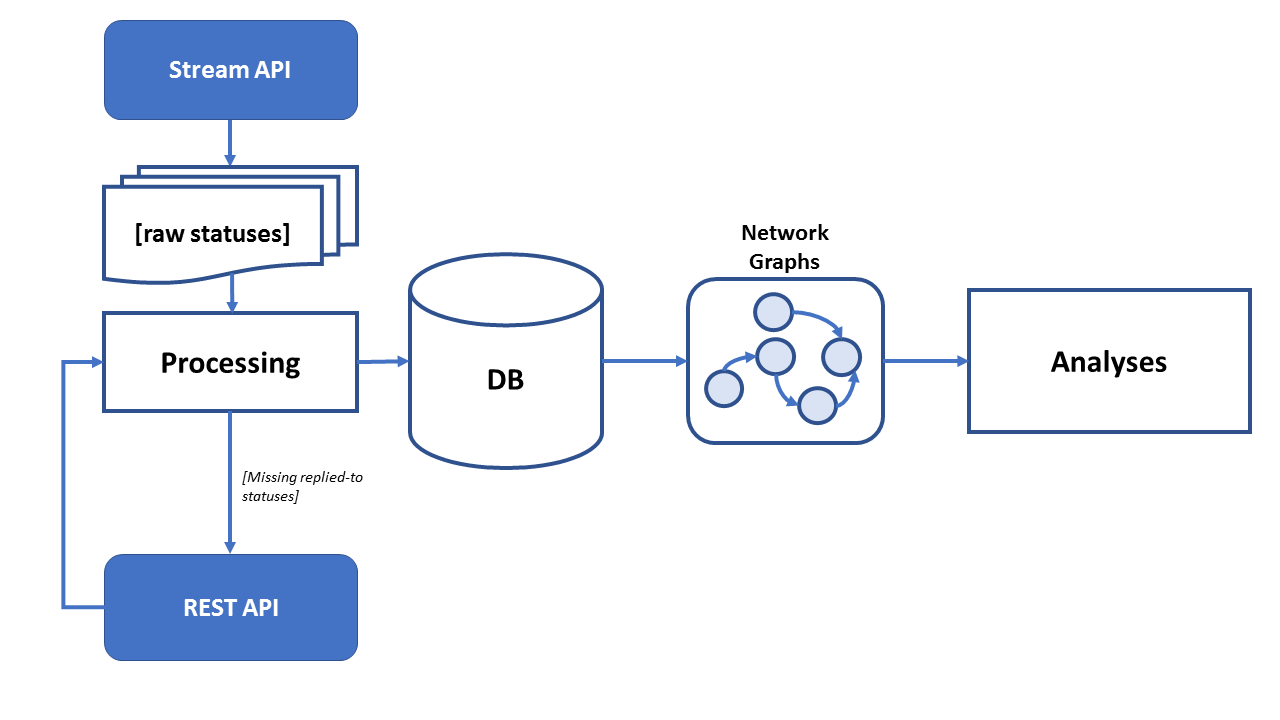
\includegraphics[width=\columnwidth]{images/frameworkstructure.png}
\caption{Overall framework structure}
\label{fig:frameworkstructure}
\end{figure}

\subsection{Streaming}

To ensure we have as much data as possible, data collection takes
three steps. First, a stream endpoint is opened to catch activities of
accounts under investigation, those accounts will be referred to as
`watched' or `CS' (Customer Service) accounts. Twitter streaming API
is designed to return tweets created by the user, their retweets,
replies to tweets created by the user, and retweets of their
tweets. However, the stream does not include tweets mentioning the
user, and replies/retweets by protected users. The first phase of data
collection phase started with collecting those activities, and has
accumulated about 15,000 tweets.

\subsection{Reply Chains}

Returned statuses from the Streaming API may represent reply to
statuses that have not been collected previously. We found that most
missing statuses were either posted before data collection started,
initial chain root that was not captured by the Stream API
(e.g. mentions), or the user account is protected. This issue could
hugely affect the data and their
analysis. Figure~\ref{fig:datacollectionphases} illustrates common
scenario that involves a group of reply chains after the phases of
data collection; sub-figure (a) shows five reply-chains that were
returned by the stream in their original structure. However, the
second phase returned one reply that connected the chains to become
one component, as shown in sub-figure (b).

Therefore, once statuses are returned from the stream endpoint, they
are processed to identify missing replied-to posts, and REST API is
used to collect them. This process is recursively done for newly
collected replies until no further replies are available. Unavailable
statuses are often result from either deletion or protected accounts.

Analysis of changes on the graph after the second phase of data
collection shows that there were increases in the number of nodes and
edges by 43\% and 62\%, respectively. This increase in connections has
resulted in merging 176 components into others, which improved
connectivity of the graph and, hence, accuracy of dependent analyses.

\begin{figure}[htb]
\centering
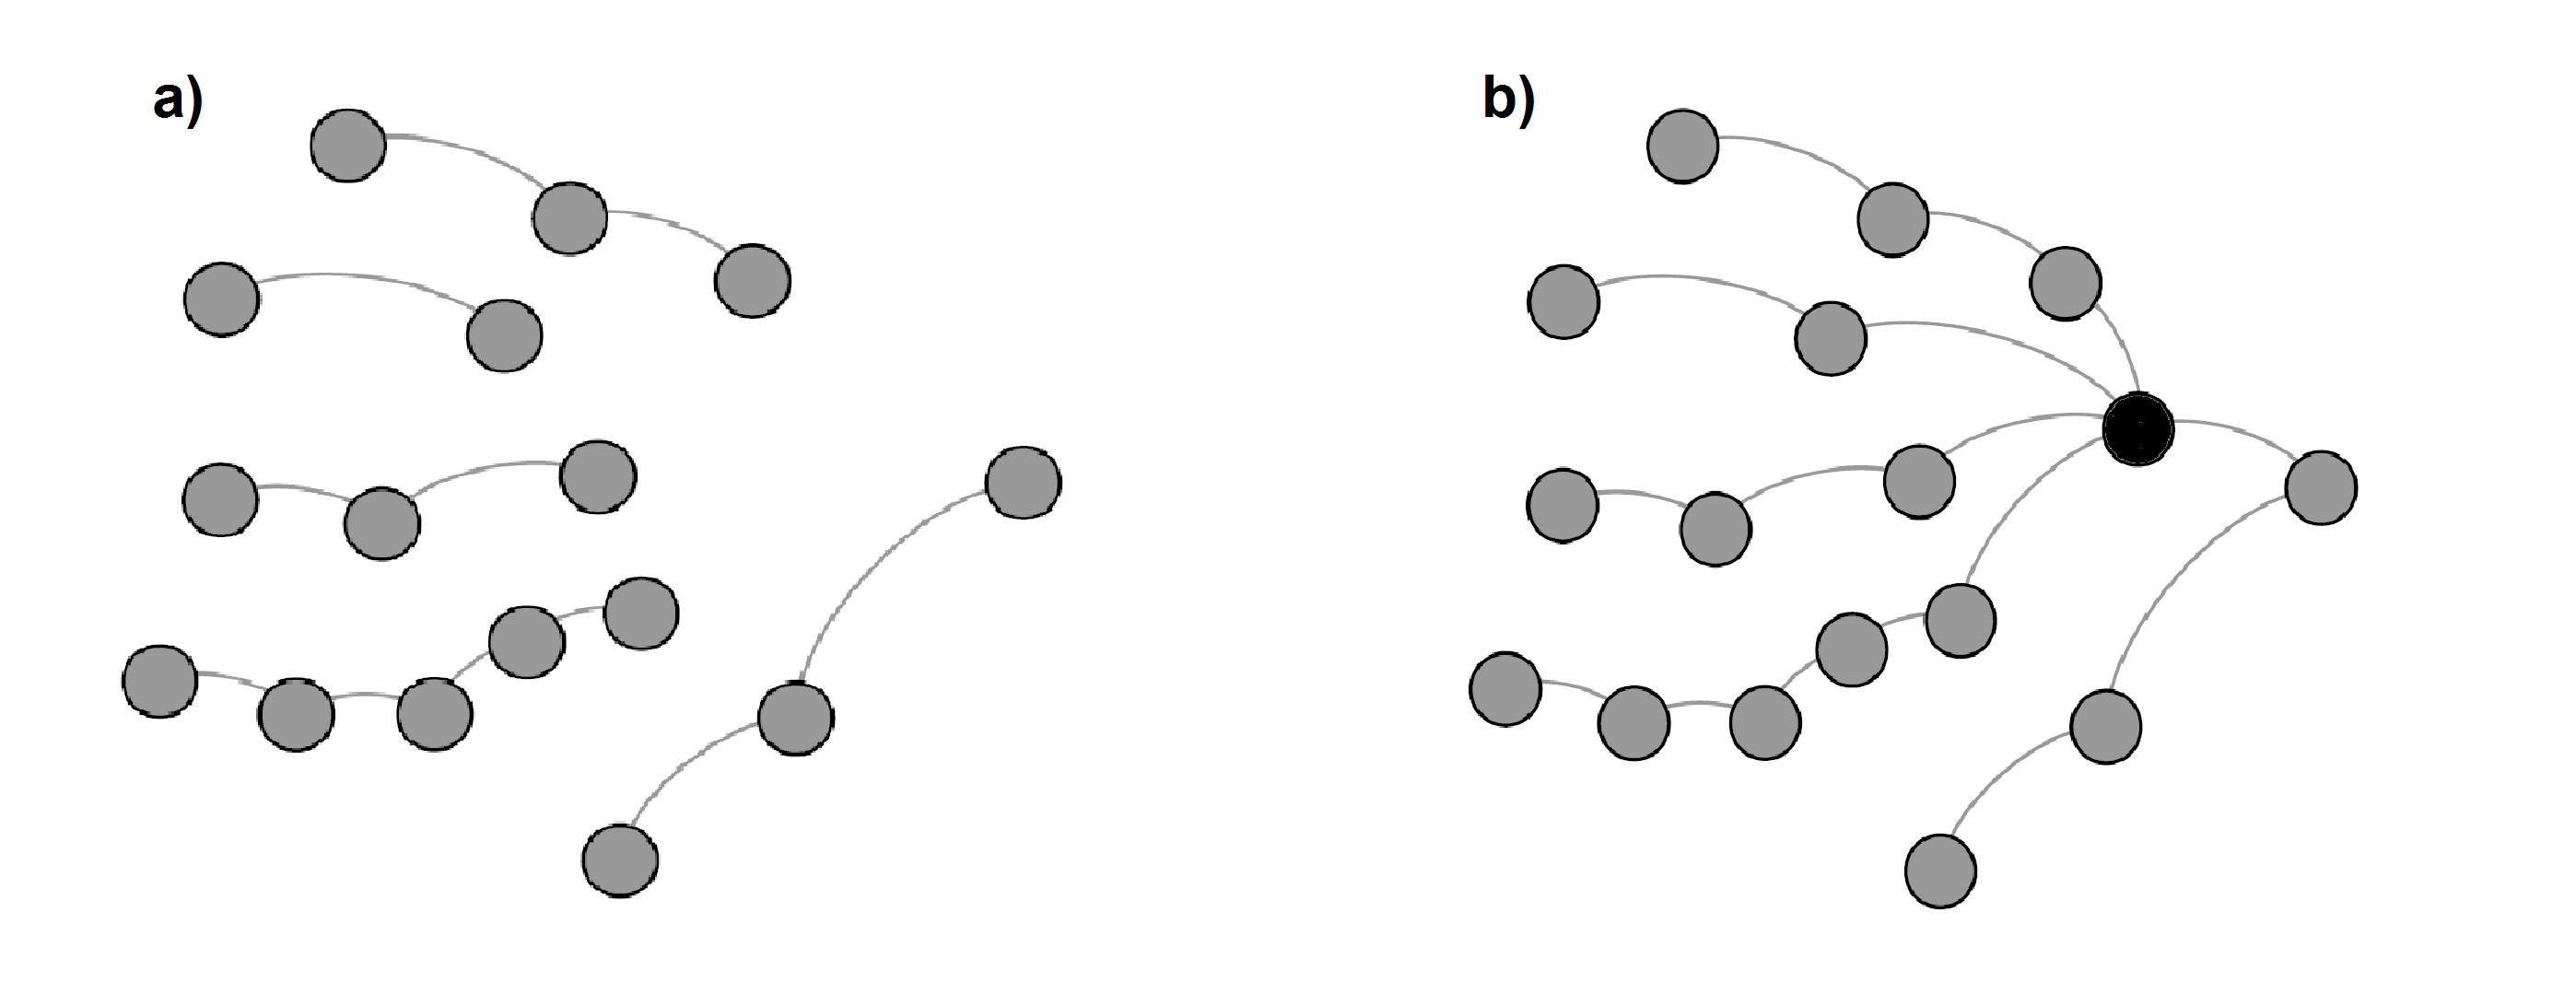
\includegraphics[width=\columnwidth]{images/datacollectionphases.png}
\caption{(a) First phase of data collection and (b) second phase of data
collection}
\label{fig:datacollectionphases}
\end{figure}


\subsection{Graph Construction}

\subsubsection{Main Graph}

Constructing graphs from the collected statuses is in core of all
analyses presented in this chapter. First, a base graph\footnote{The
terms `main graph' and `base graph' are used interchangeably.} is
generated containing all replies and the needed data. Nodes represent
post ids, while edges indicate replying direction. Other information
of statuses are added as attributes to nodes. The information used in
this study are screen name of the user, timestamp of the reply, text,
and `watched' entity, to identify CS accounts. An example graph is
shown in Figure~\ref{fig:replychaingraph}. Properties of this graph
are constrained by how replies relate to each other. In other words,
no edge is expected to have weight value other than 1. Also, no reply
status can have outdegree greater than 1, however some nodes may have
an outdegree of 0. Node with outdegree=0 can be root nodes, i.e. first
post of conversation, or they were directed to unavailable
statuses. On the other hand, indegree of nodes can be 0 or
more. Special case nodes are those with indegree and outdegree equal
to 0. Those are isolated/floating nodes and must be removed before
analysis starts. First, those nodes do not benefit the analysis as
they are not part of any conversation. Second, they will be seen as
connected component by themselves, which affects accuracy of results.

\begin{figure}[htb]
\centering
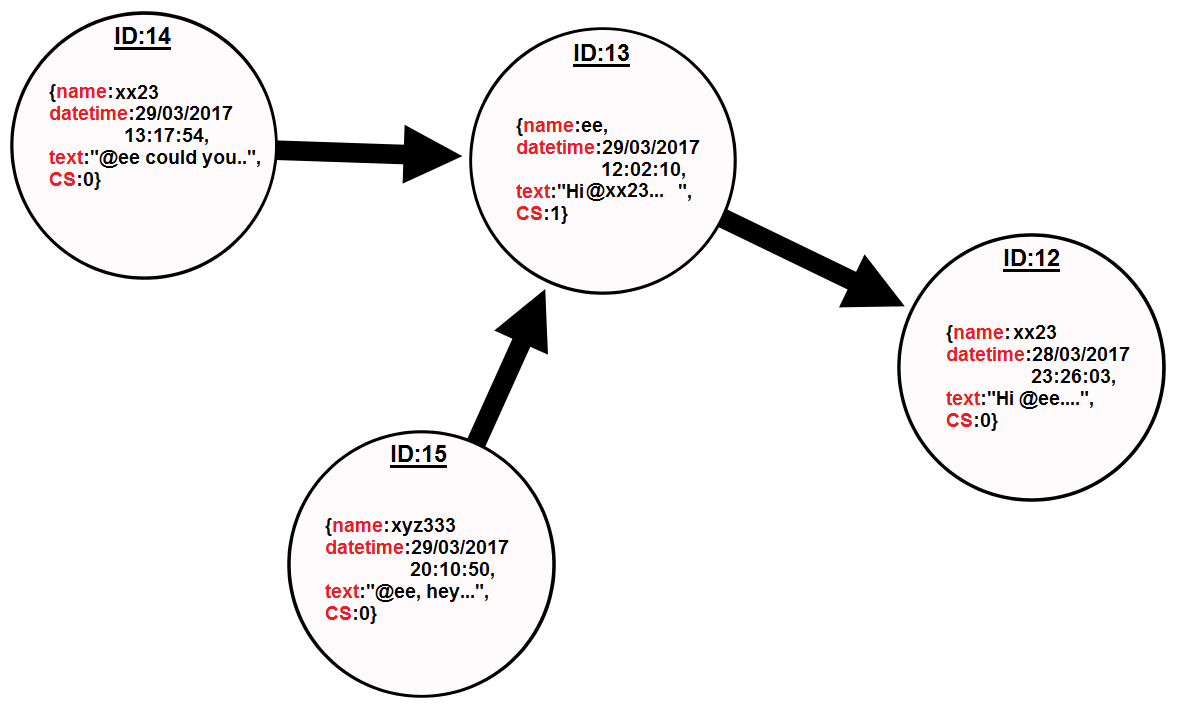
\includegraphics[width=\columnwidth]{images/replychaingraph.png}
\caption{Illustrative example of a reply chain graph and base graph}
\label{fig:replychaingraph}
\end{figure}

\subsubsection{Users' Graph}

Because most analyses focus on relationships between reply posts, they
were applied on the base graph. Nevertheless, to examine relationships
amongst users, another graph is generated from the base graph. This
process is conducted by iterating through edges linking reply posts,
extracting users' information, and constructing users graph
accordingly. Users information are embedded in node attributes. In the
perspective of this study, only two attributes are used, names and the
`watched' values. Nodes are constructed from user names, and the
attribute of `watched' is also added. For edges, their weights
indicate number of replies sent from origin node (sender) to target
node (receiver), therefore, the user graph is directed. Applying this
process on the example in Figure~\ref{fig:replychaingraph} results in
the users graph shown in Figure~\ref{fig:usersgraph}.

\begin{figure}[htb]
\centering
\includegraphics[width=\columnwidth]{images/usersgraph.png}
\caption{Example of users' graph extracted from the previous base graph}
\label{fig:usersgraph}
\end{figure}

To examine relationships between users, five network graph properties
are measured. There were no special case nodes or edges in this graph,
as observed in the base graph. Graph properties that are used in
analysing this graph and their contextual interpretations are shown in
Table ‎2.1.

\subsection{Connected Components}

The base graph consists of many number of subgraphs, each of which
represent related replies, i.e. one conversation entity. Investigating
connected components plays a major role in identifying conversations
for accounts. They are used to measure size of conversation, their
sizes/depths, and to identify shared conversations between watched
accounts. To extract conversations that user or users were engaged in,
the process iterates through nodes in each component and examine the
`name' attributes. As soon as the search is matched, no further nodes
are examined. Then, the component is either analysed on the fly, or
returned if more intensive analysis is required.

In the base graph, number of connected components reflect
conversations, while in users graph, connected components show users
communities. Therefore, in the base graph many components should be
expected, depending on activity of the watched accounts. However, in
the users graph, number of components should not exceed the number of
watched accounts, although there might be exactly one component due to
common customers.



\section{Acknowledgements}

This work has been supported by a doctoral research scholarship for
Nabeel Albishry from King Abdulaziz University, Kingdom of Saudi
Arabia.


\bibliographystyle{ACM-Reference-Format}
\bibliography{ssei2018} 

\end{document}
